%!TEX root = ../main.tex

\chapter{The background model before cuts}\label{chap:bkgbefore}

As already mentioned, a precise knowledge of background intensity and distribution is
essential to searches of faint signals. One main assumption of the \onbb-decay signal
analysis is the distribution of background events in the analysis window around \qbb\
being uniform, except for the known \Tl\ and \Bil\ \g\ lines. The primary role of the
background model is to verify this assumption by exploiting data outside this energy
region or filtered with a different event selection. The background model is also
complementary to assay measurements in determining the location of the most dangerous
background sources and learn how to improve experimental design and material selection in
similar future projects. Lastly, a good background model allows to isolate \nnbb-decay
events, estimate the half-life of the process and study their distribution as a source of
potential new-physics effects (see \cref{chap:theory}).
\newpar
A first background model has been built for the \phaseone\ data and published
in~\cite{Agostini2013a}. Later, a new and advanced model has been constructed to describe
the first 60~\kgyr\ of \phasetwo\ data before the LAr veto and PSD cuts, which has been
published in~\cite{Agostini2019b} and is described in detail in this chapter.

\section{Analysis data sets}%
\label{sec:bkg:raw:data}

\begin{table}[t]
  \small
  \centering
  \caption{%
    Properties of the data sets considered in this analysis. Further
    details about the \gerda\ detectors can be found in past
    publications~\cite{Agostini2013a, Agostini2018a}.
  }\label{tab:bkg:raw:ph2:datasets}
  \begin{tabular}{lccccc}
  \toprule
  \mr{2}{data set} & \mr{2}{composition}     & total Ge           & active \gesix\   & total Ge           & active \gesix\     \\
                   &                         & mass (kg)          & mass (kg)        & exposure (\kgyr)   & exposure (\kgyr)   \\
  \midrule
  \enrBEGeIIp\     & 29 \bege\footnotemark{} & $19.362 \pm 0.005$ & $17.17 \pm 0.32$ & $22.181 \pm 0.006$ & $17.31  \pm 0.32$  \\
  \enrSCoaxIIp\    & 6 \scoax\               & $11.827 \pm 0.002$ & $10.38 \pm 0.42$ & $13.179 \pm 0.003$ & $10.00  \pm 0.42$  \\
  \enrICoaxIIp\    & 4 \icoax\               & $ 7.802 \pm 0.002$ & $ 7.23 \pm 0.03$ & $ 8.775 \pm 0.002$ & $ 7.13  \pm 0.03$  \\
  \enrGeIIp\       & all enriched            & $38.991 \pm 0.006$ & $34.78 \pm 0.53$ & $44.135 \pm 0.007$ & $34.44  \pm 0.53$  \\
  \bottomrule
\end{tabular}

% vim: nowrap

\end{table}%
\footnotetext[1]{%
  The BEGe detector \GD{02D} is the only detector that does not fully
  deplete~\cite{Agostini2018a}. Hence, events triggered by this detector are
  not considered in either data set and it is omitted from the mass
  computation.
}

\begin{figure}
  \centering
  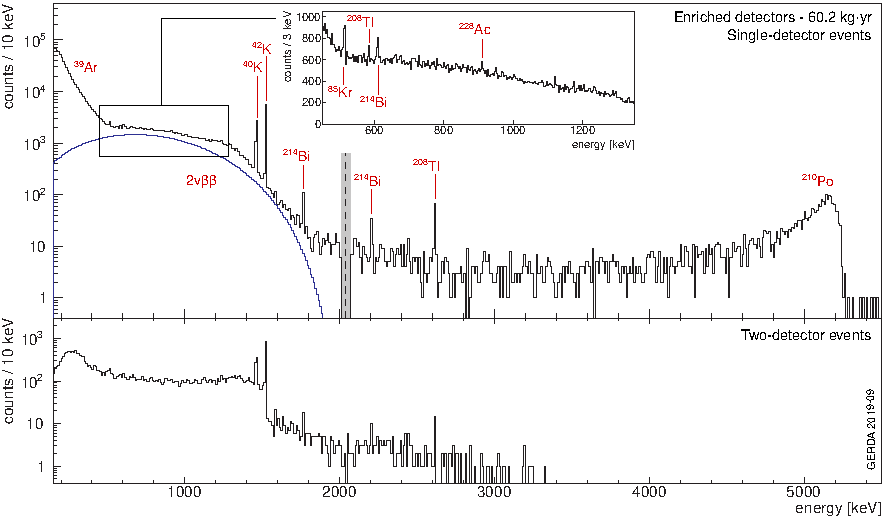
\includegraphics[width=\linewidth]{plots/bkg/raw/ph2/dataGe-desc.pdf}
  \caption{%
    Summed energy spectra of single-detector events (\enrBEGeII\ and \enrCoaxII, top
    panel) and two-detector events (\enrGeII, bottom panel) collected in \gerda\
    \phasetwo.  The prominent features due to detector intrinsic \nnbb\ events, \kvz,
    \Arl\ and \Kr\ in the LAr, \kvn, the \Thh\ and \Uh\ decay chains are highlighted. The
    window blinded for the \onbb\ analysis is marked in grey.
  }\label{fig:bkg:raw:ph2:datasets}
\end{figure}

As already mentioned, the background model before cuts has been developed using data from
the first part of \phasetwo, namely, for data acquired starting from December 2015 to
March 2018. Single-detector (or multiplicity-one, abbreviated \Mone) events and
two-detector (multiplicity-two, abbreviated \Mtwo) events are considered for this
analysis. Events from the coaxial detectors with natural isotope composition, located in
the central detector string, are not used in this analysis due to large uncertainties on
their \nplus\ contact thickness and detection efficiency. The \Mone\ events are split in
two data sets based on the two enriched detector geometries which we call \enrBEGeII\ and
\enrCoaxII\ in the following.  The \Mtwo\ data form a third data set which is named
\enrGeII. The energy we associate to an \Mtwo\ event is the sum of the energies
reconstructed in the two detectors. The data sets, their exposure and respective detector
mass are listed in \cref{tab:bkg:raw:ph2:datasets}. Note that the \bege\ exposure of
31.1~\kgyr\ is higher than the one reported in~\cite{Agostini2019a} because additional
data for which PSD methods are not applicable is here included.

The event energy distribution of the three data sets is displayed in
\cref{fig:bkg:raw:ph2:datasets}; the sum spectrum of \enrBEGeII\ and \enrCoaxII\ in the
top panel and \enrGeII\ in the bottom panel. For the single-detector data, in the top
panel, the following features are most noticeable: the \b\ decay of \Arl\ dominates the
spectrum up to 565~keV while between 600 and 1500~keV the most prominent component is the
continuous spectrum of \nnbb\ decay of \gesix. Two \g\ lines at 1461 and 1525~keV can be
attributed to \kvn\ and \kvz; further visible \g\ lines belonging to \Kr, \Tl, \Bih\ and
\Ac\ are indicated in the figure. The highest energies displayed are dominated by a
peak-like structure emerging at 5.3~MeV with a pronounced low energy tail. This is a
typical spectral feature of \a\ particles and can, here, be attributed to \Po\ decay on
the thin detector \pplus\ surfaces~\cite{Agostini2013a}.  Events above the \Po\ peak
belong to \a\ decays emerging from the \Ra\ sub-chain on the detector \pplus\ surfaces.
All these components contribute also to \enrGeII\ except for \Arl, \nnbb\ and high energy
$\alpha$-components. This is due to the short range of \a\ (tens of \mum) and \b\
particles (typically smaller than 1.5~cm) in LAr and germanium with respect to the
distance between detectors which is of the order of several cm.

% vim: tw=90
